\documentclass[11pt]{article}
\usepackage{epsfig}
\usepackage{float}
\usepackage{longtable}
\restylefloat{figure}
\restylefloat{table}
\usepackage[margin=0.75in]{geometry}
\usepackage{hyperref}
\usepackage{fancyhdr}
\pagestyle{fancy}
\lhead{PGP PPI For the RCE Gen. 3 Platform}
\rhead{Design Document}
\lfoot{Version 0.1}
\rfoot{\thepage}
\cfoot{}

\begin{document}
\thispagestyle{empty}

\title{PGP PPI For The RCE Generation 3 Platform\\Design Document}
\author{Ryan Herbst}
\date{\today}

\maketitle
\begin{table}[H]
\centering
   \begin{tabular}{| l | l | l | l | } 
      \hline \textbf{Revision} & \textbf{Effective Date} & \textbf{Description Of Changes} \\
      \hline 0.1               & \today                  & Working copy \\
      \hline
   \end{tabular}
\end{table}

\vfill
\begin{center}
SLAC National Accelerator Center
Research Engineering Division, Electronics
\end{center}
\newpage
\tableofcontents

\newpage
\listoftables

\newpage
\listoffigures



\newpage
\section{PGP PPI Modules}

\subsection{PGP PPI Top Level}
\label{subsec:pgp_ppi_top}

\subsubsection{Top Level Interfaces}

The generic ports for the top level module are shown in table \ref{tab:top_generics}. 
The exact values may expand or change depending on the implementation decisions  of the
designer. This table is meant as a guide to indicate what type of top level configurations 
may be required to meet the system requirements. 

\begin{table}[H]
\small
\centering
   \begin{tabular}{| l | l | l | l | }
      \hline \textbf{Value} & \textbf{Type} & \textbf{Default} & \textbf{Description} \\
      \hline TPD\_G                  & time    & 1 ns  & Synchronous signal delay value for simulation.       \\
      \hline LANE\_COUNT\_G     & positive & 12    & Generic to determine how many lanes are implemented. One per Lane.\\
      \hline LANEn\_RATE\_G    & TBD      & TBD   & Generics to configure the line rate of each lane. One per Lane.\\
      \hline LANEn\_WIDTH\_G   & TBD      & TBD   & Generics to configure the interface width of each lane. One per Lane.\\
      \hline LANEn\_SYNC\_G    & boolean  & false & Generics to configure enable synchronous mode for each lane. One per Lane.\\
      \hline LANEn\_VER\_G     & positive & 2     & Generics to determine the PGP version for each lane. One per Lane.\\
      \hline LANEn\_REFSEL\_G  & TBD      & TBD   & Generics to determine the reference for each lane. One per Lane.\\
      \hline
   \end{tabular}
   \caption{Top Level Generics}
   \label{tab:top_generics}
\end{table}

The proposed signal ports for the top level module are shown in table \ref{tab:top_signals}.

\begin{table}[H]
\small
\centering
   \begin{tabular}{| l | l | l | l | l | } 
      \hline \textbf{Signal}   & \textbf{Type} & \textbf{Width} & \textbf{Direction} & \textbf{Description}      \\
      \hline sysClk200         & Logic         & 1      & In        & External 200Mhz system clock. Used as the  \\
                               &               &        &           & clock for the PPI interface.              \\
      \hline sysClk200Rst      & Logic         & 1      & In        & Reset for external 200Mhz system clock.    \\
      \hline locRefClk         & Logic         & 2      & In        & Reference clocks from local DPM oscillators.\\
      \hline extRefClk         & Logic         & 3      & In        & Reference clocks from DTM.                   \\
      \hline sysClk            & Logic         & 1      & In        & System clock used by synchronous lanes.\\
      \hline sysCode           & Logic         & 8      & In        & 8-Bit system code which is forwarded by \\ 
                               &               &        &           & lanes running in synchronous mode.  \\
                               &               &        &           & Sampled when SysCodeEn is high. \\
      \hline sysCodeEn         & Logic         & 1      & In        & Enable for 8-bit system code.                         \\ 
      \hline obPpiClk          & Logic             & 1      & Out       & Outbound PPI clock input \\
      \hline obPpiToFifo       & ObPpiToFifoType   & 1      & Out       & Outbound PPI input signals \\
      \hline obPpiFromFifo     & ObPpiFromFifoType & 1      & In        & Outbound PPI output signals \\
      \hline ibPpiClk          & Logic             & 1      & Out       & Outbound PPI clock input  \\
      \hline ibPpiToFifo       & IbPpiToFifoType    & 1      & Out       & Inbound PPI input signals \\
      \hline ibPpiFromFifo     & IbPpiFromFifoType & 1      & In        & Inbound PPI output signals \\
      \hline pgpRxP            & Logic             & LANE\_COUNT\_G     & In        & PGP serial RX positive     \\
      \hline pgpRxM            & Logic             & LANE\_COUNT\_G     & In        & PGP serial RX negative     \\
      \hline pgpTxP            & Logic             & LANE\_COUNT\_G     & Out       & PGP serial TX positive     \\
      \hline pgpTxM            & Logic             & LANE\_COUNT\_G     & Out       & PGP serial TX negative     \\
      \hline
   \end{tabular}
   \caption{ArmRceG3Top Signals}
   \label{tab:top_signals}
\end{table}

\subsubsection{Top Level Block Diagram}

\begin{figure}[H]
   \centering
   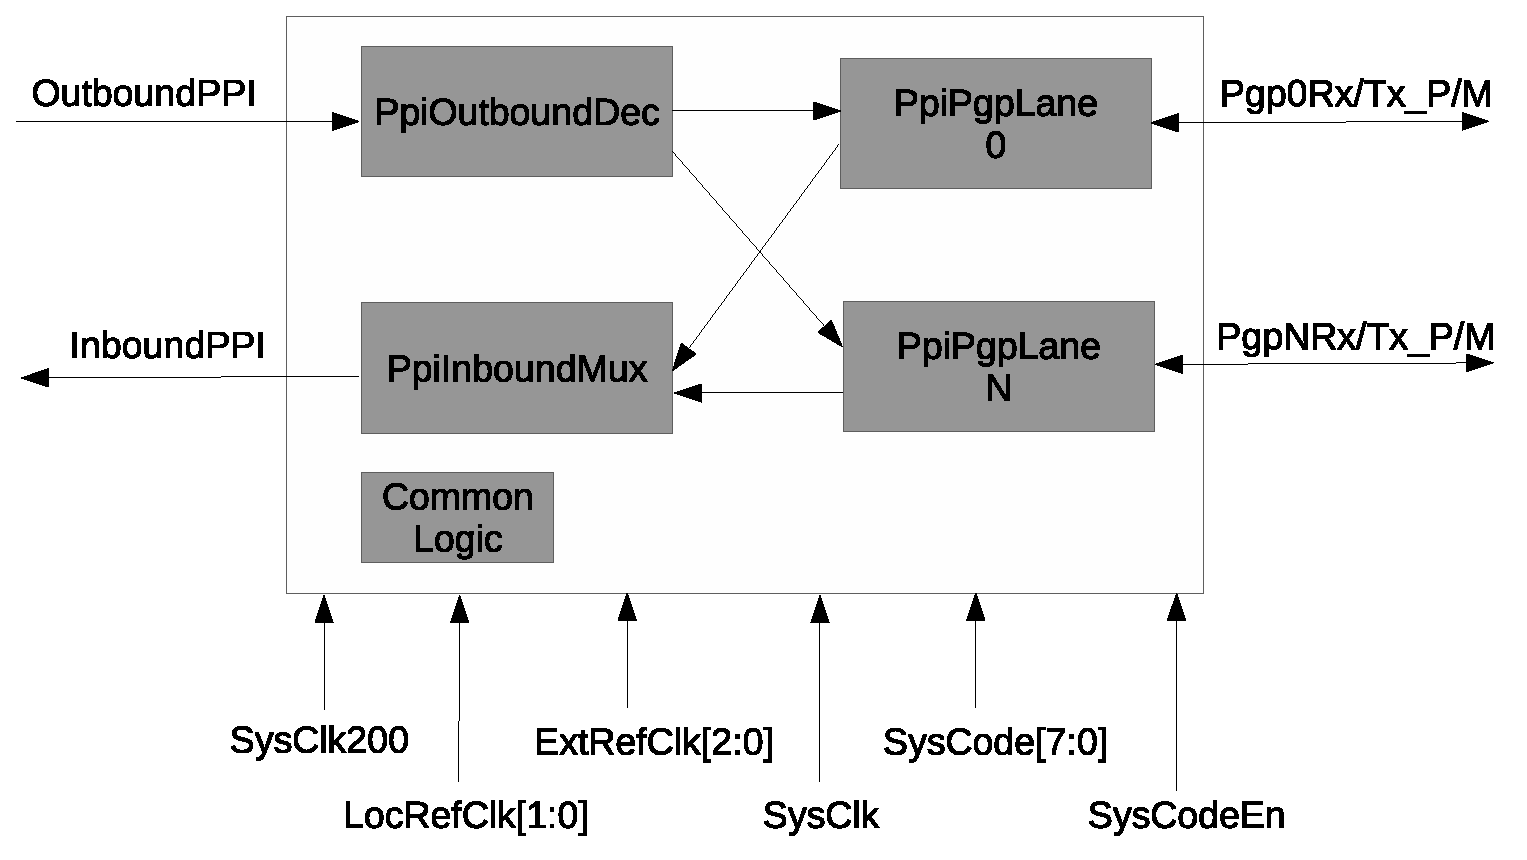
\psfig{file=images/pgp_ppi_top.eps,scale=0.50}
   \caption{Top Level Block Diagram}
   \label{fig:top_level_block}
\end{figure}

The PGP PPI block supports up to 12 PGP lanes. The 11 lanes operate independently, each having it's own width, speed, clocking
mode and version as configured through a set of generics.

\subsection{PPI Outbound Decoder}
\label{subsec:ppi_ob_dec}

The outbound decoder block serves as the interface between the single outbound PPI interface and the numerous 
PPG lane blocks. This block is implemented as a generic block which may be reused in many PPI implementations.

\subsubsection{PPI Outbound Decoder Interfaces}

The generic ports for the PPI outbound decoder module are shown in table \ref{tab:ppi_ob_dec_generics}. 
The exact values may expand or change depending on the implementation decisions  of the
designer. 

\begin{table}[H]
\small
\centering
   \begin{tabular}{| l | l | l | l | }
      \hline \textbf{Value} & \textbf{Type} & \textbf{Default} & \textbf{Description} \\
      \hline TPD\_G                  & time    & 1 ns  & Synchronous signal delay value for simulation.       \\
      \hline DEC\_COUNT\_G     & positive & 12    & Generic to determine how many decoded interfaces are implemented.\\
      \hline
   \end{tabular}
   \caption{PPI Outbound Decoder Generics}
   \label{tab:ppi_ob_dec_generics}
\end{table}

The proposed signal ports for the PPI outbound decoder module are shown in table \ref{tab:ppi_ob_dec_signals}.

\begin{table}[H]
\small
\centering
   \begin{tabular}{| l | l | l | l | l | } 
      \hline \textbf{Signal}   & \textbf{Type} & \textbf{Width} & \textbf{Direction} & \textbf{Description}      \\
      \hline obPpiClk          & Logic             & 1      & In        & Outbound PPI clock input \\
      \hline obPpiToFifo       & ObPpiToFifoType   & 1      & Out       & Outbound PPI input signals \\
      \hline obPpiFromFifo     & ObPpiFromFifoType & 1      & In        & Outbound PPI output signals \\
      \hline obDecPpiToFifo    & ObPpiToFifoType   & DEC\_COUNT\_G      & Out       & Decoded Outbound PPI input signals \\
      \hline obDecPpiFromFifo  & ObPpiFromFifoType & DEC\_COUNT\_G      & In        & Decoded Outbound PPI output signals \\
      \hline
   \end{tabular}
   \caption{PPI Outbound Decoder Signals}
   \label{tab:ppi_ob_dec_signals}
\end{table}

\subsubsection{PPI Outbound Decoder Block Diagram}

The outbound decoder block is fully synchronous to sysClk200 and does not contain any FIFOs. 
The flow control state of the destination lane determines if the frame can be read from the outbound PPI interface.

\begin{figure}[H]
   \centering
   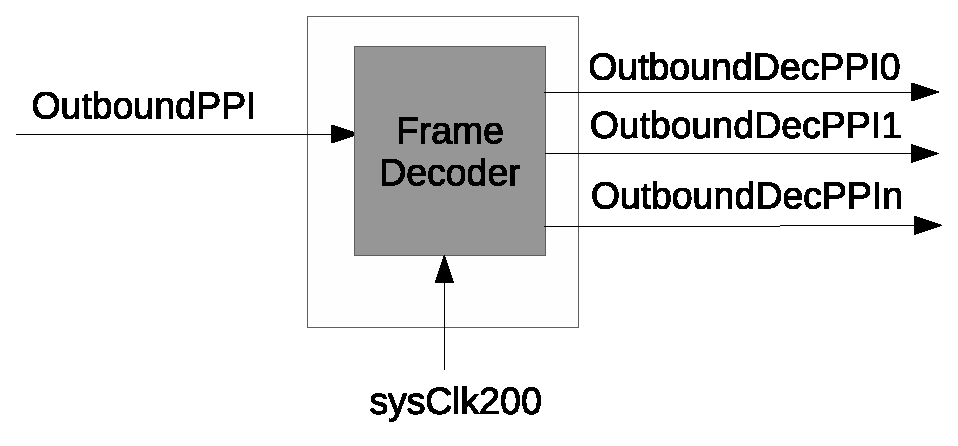
\psfig{file=images/ppi_ob_dec.eps,scale=0.50}
   \caption{PPI Outbound Decoder Block Diagram}
   \label{fig:ppi_ob_dec_block}
\end{figure}

\subsubsection{PPI Outbound Frame Format}

The following diagram shows the outbound PPI frame and the location of the field which the outbound decoder uses to direct the frame. 
The least significant byte of the first quad word transfered contains the 8-bit destination ID. 

\begin{figure}[H]
   \centering
   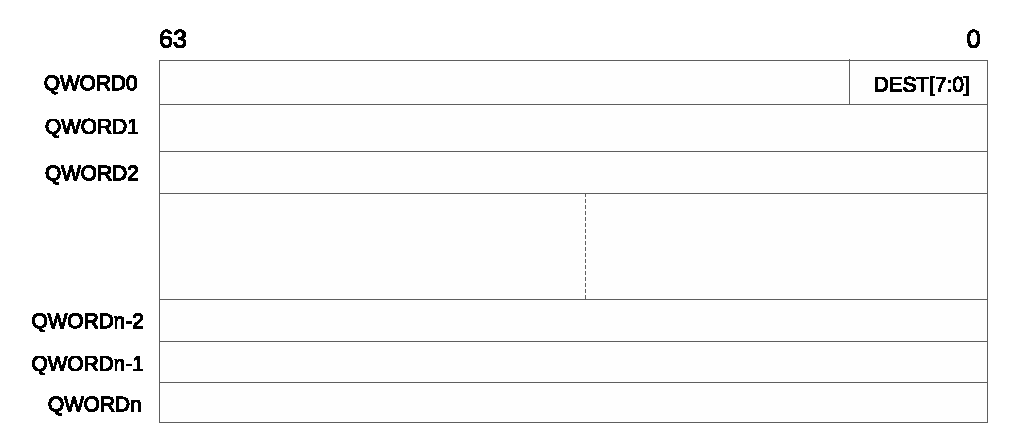
\psfig{file=images/ppi_ob_frame.eps,scale=0.50}
   \caption{PPI Outbound Decoder Frame Fields}
   \label{fig:ppi_ob_frame_fields}
\end{figure}

\subsection{PPI Inbound Multiplexer}
\label{subsec:ppi_ib_mux}

The PPI inbound multiplexer moves a frame at time from one of a number of PGP lane modules to the inbound PPI interface and is
is fully synchronous to the sysClk200 system clock. Arbitration logic chooses which lane module to accept data from while the
multiplexer moves the frame frame from the selected interface. The frame encoder updates the inbound frame indicating the source 
address of the frame. This block is implemented as a generic block which may be reused in many PPI implementations.

\subsubsection{PPI Inbound Multiplexer Interfaces}

The generic ports for the PPI inbound multiplexer module are shown in table \ref{tab:ppi_ib_mux_generics}. 
The exact values may expand or change depending on the implementation decisions  of the designer. 

\begin{table}[H]
\small
\centering
   \begin{tabular}{| l | l | l | l | }
      \hline \textbf{Value} & \textbf{Type} & \textbf{Default} & \textbf{Description} \\
      \hline TPD\_G                  & time    & 1 ns  & Synchronous signal delay value for simulation.       \\
      \hline MUX\_COUNT\_G     & positive & 12    & Generic to determine how many muliplexed interfaces are implemented.\\
      \hline
   \end{tabular}
   \caption{PPI Inbound Multiplexer Generics}
   \label{tab:ppi_ib_mux_generics}
\end{table}

The proposed signal ports for the PPI inbound multiplexer module are shown in table \ref{tab:ppi_ib_mux_signals}.

\begin{table}[H]
\small
\centering
   \begin{tabular}{| l | l | l | l | l | } 
      \hline \textbf{Signal}   & \textbf{Type} & \textbf{Width} & \textbf{Direction} & \textbf{Description}      \\
      \hline ibPpiClk          & Logic             & 1      & In        & Inbound PPI clock input \\
      \hline ibPpiToFifo       & ObPpiToFifoType   & 1      & Out       & Inbound PPI input signals \\
      \hline ibPpiFromFifo     & ObPpiFromFifoType & 1      & In        & Inbound PPI output signals \\
      \hline ibMuxPpiToFifo    & ObPpiToFifoType   & MUX\_COUNT\_G      & Out       & Multiplexed Inbound PPI input signals \\
      \hline ibMuxPpiFromFifo  & ObPpiFromFifoType & MUX\_COUNT\_G      & In        & Multiplexed Inbound PPI output signals \\
      \hline laneReq           & Logic              & MUX\_COUNT\_G     & In        & Lane frame request.             \\
      \hline laneGnt           & Logic              & MUX\_COUNT\_G     & Out       & Lane frame grane.             \\
      \hline
   \end{tabular}
   \caption{PPI Inbound Multiplexer Signals}
   \label{tab:ppi_ib_mux_signals}
\end{table}

\subsubsection{PPI Inbound Multiplexer Block Diagram}

The inbound multiplexer block is fully synchronous to sysClk200 and does not contain any FIFOs.

\begin{figure}[H]
   \centering
   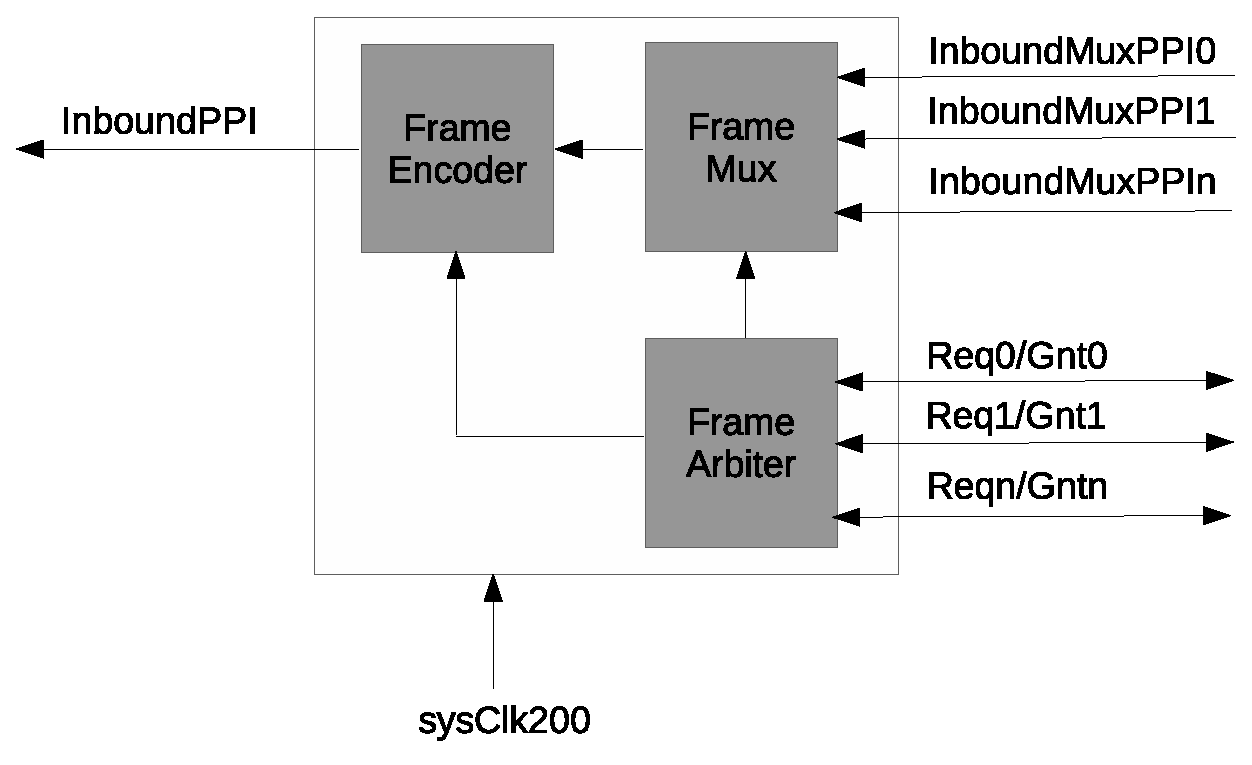
\psfig{file=images/ppi_ib_mux.eps,scale=0.50}
   \caption{PPI Inbound Multiplexer Block Diagram}
   \label{fig:ppi_ib_mux_block}
\end{figure}

\subsubsection{PPI Inbound Frame Format}

The following diagram shows the inbound PPI frame and the location of the field into which the frame source is encoded.
The least significant byte of the first quad word transfered contains the 8-bit source ID. 

\begin{figure}[H]
   \centering
   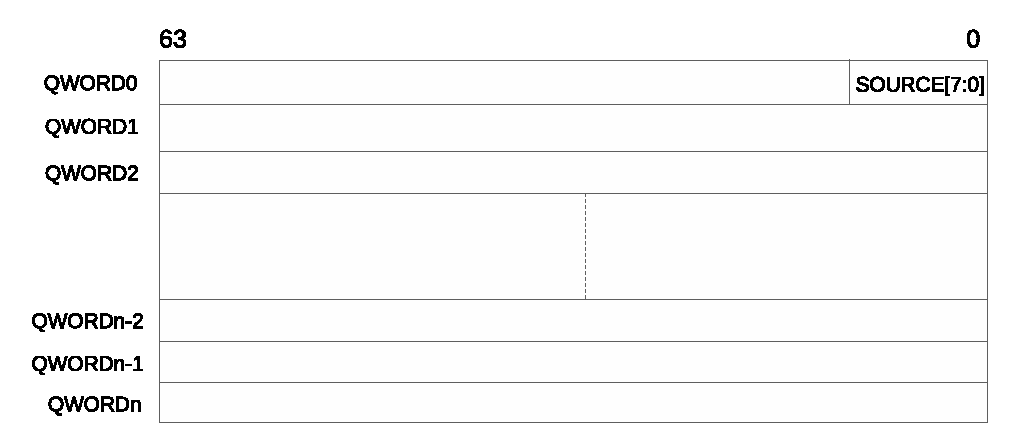
\psfig{file=images/ppi_ib_frame.eps,scale=0.50}
   \caption{PPI Inbound Multiplexer Frame Fields}
   \label{fig:ppi_ib_frame_fields}
\end{figure}

\subsection{PPI PGP Lane Module}
\label{subsec:ppi_pgp_lane}

The PGP lane module contains the logic required to interface a single PGP lane with the inbound and outbound PPI interfaces.
This module is designed to be generic with numerous variations supporting configurable modes and versions of the PGP cores.

\subsubsection{PPI PGP Lane Interfaces}

The generic ports for the PPI PGP lane module are shown in table \ref{tab:ppi_pgp_lane_generics}. 
The exact values may expand or change depending on the implementation decisions  of the designer. 

\begin{table}[H]
\small
\centering
   \begin{tabular}{| l | l | l | l | }
      \hline \textbf{Value} & \textbf{Type} & \textbf{Default} & \textbf{Description} \\
      \hline TPD\_G                  & time    & 1 ns  & Synchronous signal delay value for simulation.       \\
      \hline LANE\_RATE\_G    & TBD      & TBD   & Generics to configure the line rate of the lane. \\
      \hline LANE\_WIDTH\_G   & TBD      & TBD   & Generics to configure the interface width of the lane. \\
      \hline LANE\_SYNC\_G    & boolean  & false & Generics to configure enable synchronous mode for the lane. \\
      \hline LANE\_VER\_G     & positive & 2     & Generics to determine the PGP version for the lane. \\
      \hline LANE\_REFSEL\_G  & TBD      & TBD   & Generics to determine the reference for the lane. \\
      \hline
   \end{tabular}
   \caption{PPI PGP Lane Generics}
   \label{tab:ppi_pgp_lane_generics}
\end{table}

The proposed signal ports for the PPI PGP Lane module are shown in table \ref{tab:ppi_pgp_lane_signals}.

\begin{table}[H]
\small
\centering
   \begin{tabular}{| l | l | l | l | l | } 
      \hline \textbf{Signal}   & \textbf{Type} & \textbf{Width} & \textbf{Direction} & \textbf{Description}      \\
      \hline sysClk200         & Logic         & 1      & In        & External 200Mhz system clock. Used as the  \\
                               &               &        &           & clock for the PPI interface.              \\
      \hline sysClk200Rst      & Logic         & 1      & In        & Reset for external 200Mhz system clock.    \\
      \hline locRefClk         & Logic         & 2      & In        & Reference clocks from local DPM oscillators.\\
      \hline extRefClk         & Logic         & 3      & In        & Reference clocks from DTM.                   \\
      \hline sysClk            & Logic         & 1      & In        & System clock used by synchronous lanes.\\
      \hline sysCode           & Logic         & 8      & In        & 8-Bit system code which is forwarded by \\ 
                               &               &        &           & lane when running in synchronous mode.  \\
                               &               &        &           & Sampled when SysCodeEn is high. \\
      \hline sysCodeEn         & Logic         & 1      & In        & Enable for 8-bit system code.                         \\ 
      \hline obPpiToFifo       & ObPpiToFifoType   & 1      & Out       & Outbound PPI input signals \\
      \hline obPpiFromFifo     & ObPpiFromFifoType & 1      & In        & Outbound PPI output signals \\
      \hline ibPpiToFifo       & IbPpiToFifoType    & 1      & Out       & Inbound PPI input signals \\
      \hline ibPpiFromFifo     & IbPpiFromFifoType & 1      & In        & Inbound PPI output signals \\
      \hline laneReq           & Logic              & 1      & Out       & Lane frame request.             \\
      \hline laneGnt           & Logic              & 1      & In        & Lane frame grane.             \\
      \hline pgpRxP            & Logic             & 1    & In        & PGP serial RX positive     \\
      \hline pgpRxM            & Logic             & 1  & In        & PGP serial RX negative     \\
      \hline pgpTxP            & Logic             & 1   & Out       & PGP serial TX positive     \\
      \hline pgpTxM            & Logic             & 1    & Out       & PGP serial TX negative     \\
      \hline
   \end{tabular}
   \caption{PPI PGP Lane Signals}
   \label{tab:ppi_pgp_lane_signals}
\end{table}

\subsubsection{PPI PGP Lane Block Diagram}

The proposed block diagram for the PPI PGP Lane module is shown below. The logic is separated into blocks which are each 
described in detail in the following text. The PPI PGP lane module has a number of input clocks to support a wide variety of operating
modes. The inbound and outbound PPI interfaces are synchronous to sysClk200 
One of the other inputs clocks is chosen to be the reference clock for the PGP module depending on the chosen operating mode. 
SysClk, sysCode and sysCodeEn are utilized for the PGP module operating in synchronous mode while the remaining 
reference clocks are available when operating in asynchronous mode.

\begin{figure}[H]
   \centering
   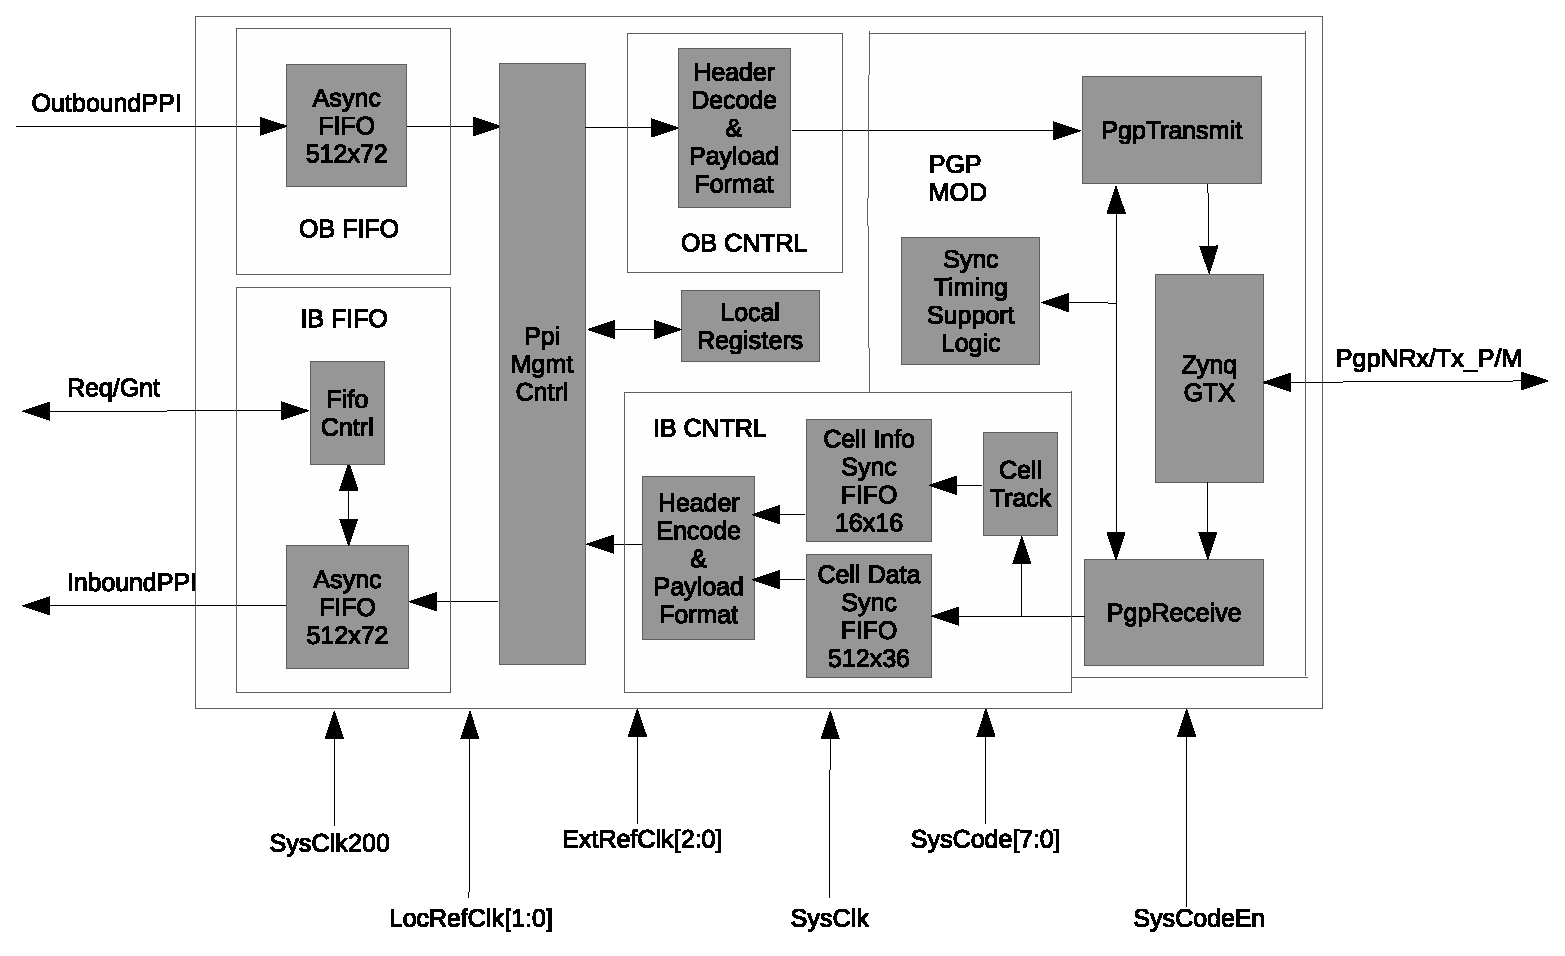
\psfig{file=images/ppi_pgp_lane.eps,scale=0.75}
   \caption{PPI PGP Lane Block Diagram}
   \label{fig:ppi_pgp_lane_block}
\end{figure}

\subsubsection{Outbound FIFO Block}

The outbound FIFO block (OB FIFO) receives outbound PPI frames from the outbound PPI decoder module. Data is buffered in an asynchronous 
72-bit x 512 entry FIFO with the PPI side being synchronous to SysClk200 and the PGP side being synchronous to the
configured PGP transmit clock. The output of this FIFO is passed to the PPI management control module.

\subsubsection{PPI Management Control}

The PPI management control module (see section \ref{subsec:PpiMgmtCntrl}) sits in both the outbound and inbound data paths. 
This module intercepts and processes management frames that are received at the outbound PPI interface. 

\subsubsection{Outbound Control}

The outbound control block (OB CNTRL) receives the PPI frame, decodes the header and passes the payload to the appropriate PGP virtual
channel. The 64-bit words received from the PPI interface are passed to the PGP transmit core in smaller units containing
16-bits or 32-bits of data as determined by the native width of the configure PGP transmit core with the lower bits being
transmitted first.  The EOF and size fields of the outbound PPI frame indicate the end of the transmitted cell. 

This module monitors the flow control signals for the selected virtual channel, pausing data transmission as necessary.

All of the logic in the outbound control block is synchronous to the PGP transmit clock.

The following diagram shows the proposed format for the outbound PGP frame. The first 64-bit quad word forms the header and
contains control information for the outbound frame.

\begin{figure}[H]
   \centering
   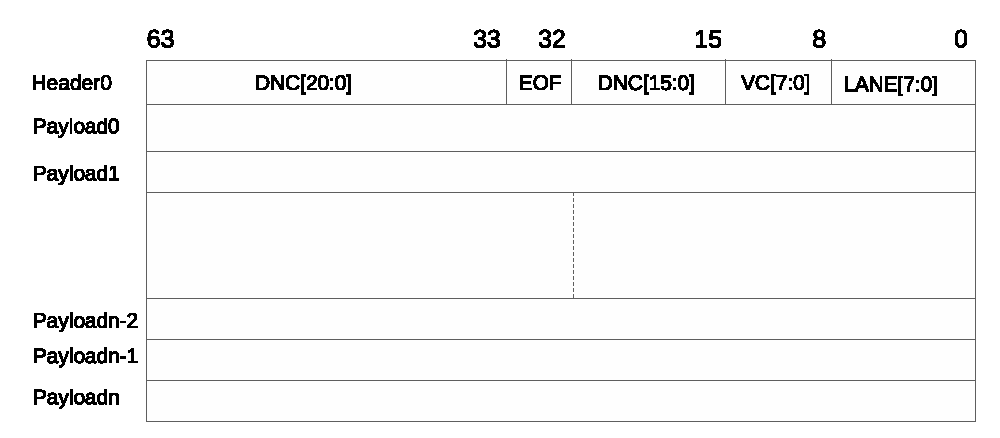
\psfig{file=images/ppi_ob_lane_frame.eps,scale=0.75}
   \caption{PPI PGP Outbound Frame Format}
   \label{fig:ppi_ob_lane_frame}
\end{figure}

The following fields are found in the outbound PPI header word:

\begin{itemize}
   \item Lane[7:0]: Identifies the destination lane for the outbound frame. (ignored by this block)
   \item VC[7:0]: Identifies the destination virtual channel for the outbound frame.
   \item EOF: Indicates if this cell is the last in a frame.
\end{itemize}

\subsubsection{PGP Module}

The PGP module (PGP MOD) contains the generic PGP core and it's support logic. This block of logic is implemented using one of the
PGP modules provided by the PGP support library. This block contains the receive and transmit PGP cores, the Zynq GTX module 
and additional logic required to support synchronous clocking. The details of this module are described in a separate
document. 

The interface to PGP module will include a number of configuration and status vectors which must be supported by the local register logic.

\subsubsection{Inbound Control}

The inbound controller (IB CNTRL) will receive partial frames from the PGP receive core. Each of these partial frames contains a 
a single PGP cell worth of data. The boundary between receive cells is indicated when the valid signal is 
de-asserted by the PGP receive core. All of the logic in the inbound control block is synchronous to the PGP receive clock.

Received cell data is passed directly to the cell data buffer which is implemented in a 36-bit by 512 entry FIFO. This FIFO
is 36-bits wide in order to support future versions of the PGP core which will utilize a 32-bit wide interface. The upper half of this 
FIFO is not be utilized when interfacing to the current 16-bit PGP cores.

When the end of the cell is received the cell tracking logic will add a single 16-bit entry to the cell information buffer. This buffer is
implemented in a synchronous distributed ram 16-bit x 16-entry FIFO. This buffer stores information about the length, virtual channel
and control signals (EOF and EOFE) of the received cell. 

The header encode and payload format block of firmware will pull entries from the cell information and cell data FIFOs. The entries from
these two FIFOs are used to form the inbound PPI frame as shown in the following diagram. The frame is then passed through the PpiMgmtCntrl 
block and on to the inbound PPI FIFO control block. This block forms the received 16-bit (or 32-bit) PGP data into 64-bit quad words for
the PPI inbound interface.  The lower 16-bits of the 64-bit quad word are filled first. The EOF bit and size field of the inbound PPI 
interface are updated accordingly and a single idle cycle is inserted between each inbound PPI frame.

\begin{figure}[H]
   \centering
   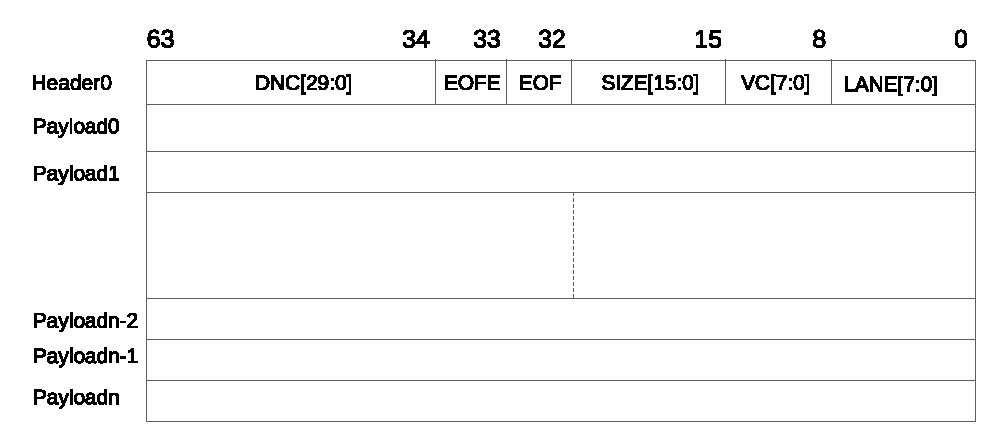
\psfig{file=images/ppi_ib_lane_frame.eps,scale=0.75}
   \caption{PPI PGP Inbound Frame Format}
   \label{fig:ppi_ib_lane_frame}
\end{figure}

The following fields are found in the inbound PPI header word:

\begin{itemize}
   \item Lane[7:0]: Identifies the source lane for the outbound frame. (set to zero by this block)
   \item VC[7:0]: Identifies the source virtual channel for the outbound frame.
   \item Size[15:0]: Indicates the size of the received cell in bytes.
   \item EOF: Indicates that the cell received is the last in a PGP frame.
   \item EOFE: Indicates that the frame contained errors (coincident with EOF).
\end{itemize}

The inbound control block will assert flow control to the PGP core based upon the fill level of the cell information and cell data FIFOs. 

\subsubsection{Inbound PPI FIFO}

The inbound PPI FIFO logic (IB FIFO) accepts inbound cell frame from the inbound controller as well as management response frames generated in the
PPI management control module. Inbound PPI frames are buffered in an asynchronous 72-bit x 512 entry FIFO. The PGP side of this
FIFO is synchronous to the PGP receive clock while the PPI side of this FIFO is synchronous to SysClk200. 

The FIFO control logic contained within this block keeps track of the number of PPI frames stored in the asynchronous FIFO. If at least
one frame exists in this FIFO it will assert the request line to the inbound PPI multiplexer logic. When the incoming grant line is
asserted, a single frame of data will be read out of the FIFO to the inbound PPI multiplexer. The request line is de-asserted between
each frame to allow for re-arbitration.

\subsection{PPI Management Module}
\label{subsec:PpiMgmtCntrl}

The PPI management module is designed to interface with both the receive and transmit data paths. This module intercepts management
frames sourced from the outbound PPI interface and converts them into local register read and write transactions. In the
inbound direction response frames are inserted into the inbound data paths when gaps permit. The PPI management block
supports three separate clock domains, one for the outbound data path, one for the inbound data path and the last for the local
register bus.

This module is designed to be generic and used in a number of PPI implementations.

\subsubsection{PPI Management Interfaces}

The generic ports for the PPI management module are shown in table \ref{tab:ppi_mgmt_generics}. 
The exact values may expand or change depending on the implementation decisions  of the designer. 

\begin{table}[H]
\small
\centering
   \begin{tabular}{| l | l | l | l | }
      \hline \textbf{Value} & \textbf{Type} & \textbf{Default} & \textbf{Description} \\
      \hline TPD\_G                  & time    & 1 ns  & Synchronous signal delay value for simulation.       \\
      \hline
   \end{tabular}
   \caption{PPI Management Generics}
   \label{tab:ppi_mgmt_generics}
\end{table}

The proposed signal ports for the PPI management module are shown in table \ref{tab:ppi_mgmt_signals}.

\begin{table}[H]
\small
\centering
   \begin{tabular}{| l | l | l | l | l | } 
      \hline \textbf{Signal}   & \textbf{Type} & \textbf{Width} & \textbf{Direction} & \textbf{Description}      \\
      \hline obPpiClock        & Logic             & 1      & In        & Outbound PPI clock \\
      \hline obPpiToFifo       & ObPpiToFifoType   & 1      & Out       & Outbound PPI input signals \\
      \hline obPpiFromFifo     & ObPpiFromFifoType & 1      & In        & Outbound PPI output signals \\
      \hline obLocPpiToFifo    & ObPpiToFifoType   & 1      & In        & Local Outbound PPI input signals \\
      \hline obLocPpiFromFifo  & ObPpiFromFifoType & 1      & Out       & Local Outbound PPI output signals \\
      \hline ibPpiClock        & Logic             & 1      & In        & Inbound PPI clock \\
      \hline ibPpiToFifo       & IbPpiToFifoType    & 1      & Out       & Inbound PPI input signals \\
      \hline ibPpiFromFifo     & IbPpiFromFifoType & 1      & In        & Inbound PPI output signals \\
      \hline ibLocPpiToFifo    & IbPpiToFifoType    & 1      & In        & Local Inbound PPI input signals \\
      \hline ibLocPpiFromFifo  & IbPpiFromFifoType & 1      & Out       & Local Inbound PPI output signals \\
      \hline regClock          & Logic             & 1      & In        & Local register space clock \\
      \hline regAddr           & Logic             & 16     & Out       & Local register address bus \\
      \hline regWriteEnable    & Logic             & 1      & Out       & Local register write enable signal \\
      \hline regWriteData      & Logic             & 32     & Out       & Local register write data bus  \\
      \hline regReadEnable     & Logic             & 1      & Out       & Local register read enable signal \\
      \hline regReadValid      & Logic             & 1      & In        & Local register read data valid signal \\
      \hline regReadData       & Logic             & 32     & In        & Local register read data bus \\
      \hline 
   \end{tabular}
   \caption{PPI Management Signals}
   \label{tab:ppi_mgmt_signals}
\end{table}

\subsubsection{PPI Management Block Diagram}

The following block diagram shows the internal structure of the PPI management block. Two asynchronous FIFOs
of undetermined size are used to buffer incoming requests and outgoing responses.

\begin{figure}[H]
   \centering
   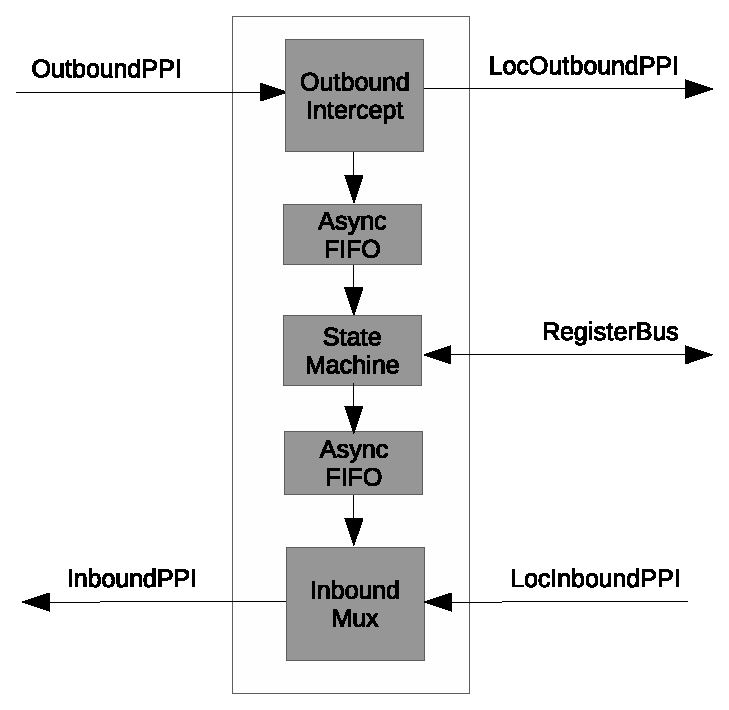
\psfig{file=images/ppi_mgmt_block.eps,scale=0.50}
   \caption{PPI Management Block Diagram}
   \label{fig:ppi_mgmt_block}
\end{figure}

\subsubsection{PPI Management Frames}

The following figure shows the format for an outbound management frame. This frame contains a single 64-bit quad word header
containing the lane number (updated and decoded by external blocks), a write enable bit, a 16-bit address and 32-bit data.

Read requests have the write bit set to zero and an empty data field. Once the read transaction has completed the frame will be
sent back to the PPI software with the data field containing the resulting read data.

Write requests will have the write bit set to one and contain the write data. The write transaction is processed without a
response?

\begin{figure}[H]
   \centering
   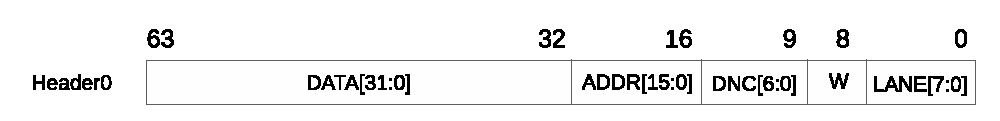
\psfig{file=images/ppi_mgmt_frame.eps,scale=0.75}
   \caption{PPI PGP Management Frame}
   \label{fig:ppi_mgmt_frame}
\end{figure}

\subsubsection{Local Register Bus}

An example write transaction is shown in the following figure. The address, write enable and write data are presented for a single clock
period.

\begin{figure}[H]
   \centering
   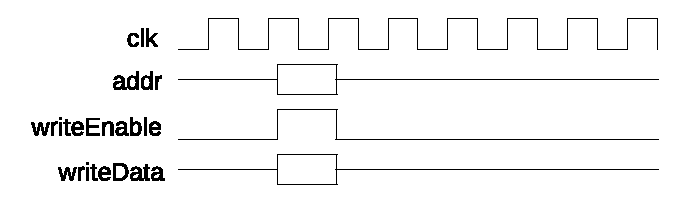
\psfig{file=images/ppi_mgmt_write.eps,scale=0.50}
   \caption{PPI PGP Management Write}
   \label{fig:ppi_mgmt_write}
\end{figure}

An example read transaction is shown in the following figure. The address and read enable signal are asserted for a single clock period.
The state machine then waits for the local bus client to return the read data on the readData vector coincident with the assertion 
of the readValid signal. The state machine will wait for up to 256 clock cycles for the local bus slave to complete the read transaction. 
If the local bus slave does not respond within this period of time the transaction will be terminated and the read data returned will be 
0xdeadbeef. 

\begin{figure}[H]
   \centering
   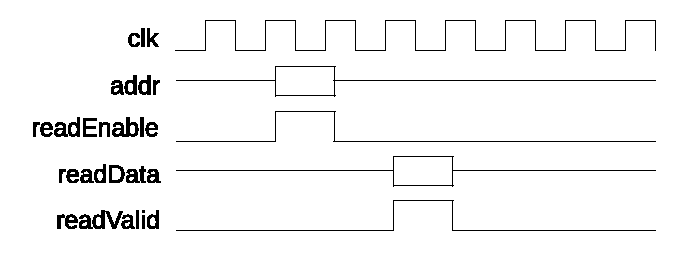
\psfig{file=images/ppi_mgmt_read.eps,scale=0.50}
   \caption{PPI PGP Management Read}
   \label{fig:ppi_mgmt_read}
\end{figure}

\end{document}

